%---------- Inleiding ---------------------------------------------------------

\section{Inleiding}%
\label{sec:inleiding}
De explosieve groei van data en de toenemende vraag naar naadloze integraties tussen applicaties hebben de rol van Application Programming Interfaces (API's) centraal geplaatst in de hedendaagse softwareontwikkeling. Een goed ontworpen en gedocumenteerde API is niet langer een luxe, maar essentieel voor succes in het digitale landschap. Dit is met name relevant voor BrightAnalytics, een bedrijf dat een geavanceerd data-visualisatieplatform aanbiedt voor financiële rapportering en business intelligence. De kwaliteit, consistentie en efficiëntie van de API's die BrightAnalytics ontwikkelt, zijn van cruciaal belang voor de functionaliteit van hun producten, de integratie met andere systemen en het snel kunnen ontwikkelen van nieuwe features.

\bigskip

Tijdens mijn stage bij BrightAnalytics ontwikkel ik "BrightEats", een applicatie waarmee werknemers hun lunch kunnen bestellen. Deze applicatie is afhankelijk van een backend API, geschreven in Laravel, net zoals alle andere applicaties bij BrightAnalytics. De ontwikkeling van deze API biedt een uitgelezen kans om de principes van RESTful API design te implementeren en om te evalueren welke voor- en nadelen de meer geavanceerde principes hiervan (met name OpenAPI en Hypermedia As The Engine Of Application State (HATEOAS) ) met zich meebrengen.

\bigskip

Het principe van RESTful API design werd in 2000 geïntroduceerd door Roy Fielding in zijn proefschrift \autocite{Fielding2000}. REST (Representational State Transfer) is ondertussen wijdverspreid en wordt goed ondersteund wanneer we een API willen bouwen met Laravel. Echter zijn de meer geavanceerde onderdelen van REST, met name HATEOAS (Hypermedia As The Engine Of Application State) en OpenAPI, minder bekend en worden ze minder vaak toegepast in de praktijk. Deze principes kunnen echter een grote impact hebben op de kwaliteit, consistentie en onderhoudbaarheid van een API.

\bigskip

Met deze bachelorproef proberen we een antwoord te formuleren op de volgende onderzoeksvraag:

\begin{center}
\textbf{Welke concrete voordelen biedt de implementatie van RESTful API design, en in het bijzonder HATEOAS en OpenAPI, voor de kwaliteit, consistentie en onderhoudbaarheid van een Laravel-API en een bijbehorende frontend applicatie?}
\end{center}

\bigskip

We moeten hiervoor volgende deelvragen beantwoorden:

\begin{itemize}
  \item Wat zijn de principes van RESTful API design en hoe dragen deze bij aan betere API's?
  \item Wat is HATEOAS en hoe kan dit principe worden toegepast in een Laravel-API?
  \item Wat is OpenAPI en hoe kan dit worden toegepast in de documentatie van een Laravel-API?
  \item Welke concrete voordelen biedt de implementatie van deze principes voor de kwaliteit, consistentie en onderhoudbaarheid van de BrightEats API?
  \item Hoeveel aanpassingen zijn er nodig in de frontend applicatie om te kunnen werken met een HATEOAS API? Draagt dit bij aan de onderhoudbaarheid van deze applicatie?
\end{itemize}

Deze vragen zullen beantwoord worden aan de hand van de volgende onderzoeksdoelstellingen:

\bigskip

\begin{enumerate}
\item \textbf{Inzicht verwerven in RESTful API design:} Een diepgaande analyse van de principes van RESTful API design, HATEOAS en OpenAPI specificatie, om deze zo goed mogelijk te kunnen toepassen en evalueren. We gaan ook na hoe we dit kunnen implementeren in een Laravel-API.
\item \textbf{Ontwikkeling API en bijbehorende front-end:} Het ontwikkelen en refactoren van de BrightEats API naar deze standaarden om zo de voor- en nadelen te kunnen evalueren. Hierbij gaan we ook de impact op de frontend applicatie evalueren.
\item \textbf{Formuleren van aanbevelingen:} Op basis van de bevindingen tijdens de implementatie nagaan welke principes van RESTful API design, HATEOAS en OpenAPI nuttig zijn voor BrightAnalytics en hoe deze best kunnen worden toegepast in de praktijk.
\end{enumerate}

\bigskip

Deze bachelorproef is relevant voor BrightAnalytics, omdat we kunnen nagaan of het implementeren van HATEOAS en OpenAPI in API's effectief een meerwaarde biedt. Ook is het interessant om na te gaan welke kosten en moeite er gepaard gaan met het implementeren van deze principes en of deze opwegen tegen de voordelen. Hoe compatibel zijn deze principes met de tech stack (Laravel, Vue.js) van BrightAnalytics en welke best practices kunnen worden geformuleerd voor de implementatie hiervan?

\section{Literatuurstudie}%
\label{sec:literatuurstudie}

REST (Representational State Transfer) is een veelgebruikte architectuur om API's te ontwerpen en bouwen \autocite{Eddouibi2017}. Die populariteit heeft REST te danken aan zijn eenvoud, schaalbaarheid en compatibiliteit met de standaarden van het internet. Dankzij REST kunnen ontwikkelaars op een flexibele en efficiënte manier API's bouwen die vlot kunnen omgaan met de almaar toenemende hoeveelheid data die bedrijven vandaag genereren. In de volgende secties zullen we dieper ingaan op de principes en voordelen van RESTful API's.

\subsection{De principes van RESTful API's}

RESTful API's zijn gebaseerd op een aantal belangrijke principes die bijdragen aan hun eenvoud, schaalbaarheid en gebruiksvriendelijkheid. Eén van die principes is de client-server architectuur \autocite{Fielding2000}. Een RESTful API maakt een duidelijke scheiding tussen de client, die een aanvraag doet (bijvoorbeeld een rapport opvragen), en de server, die de aanvraag verwerkt en een antwoord terugstuurt. Deze scheiding zorgt ervoor dat de client en server onafhankelijk van elkaar kunnen evolueren, wat de flexibiliteit en onderhoudbaarheid ten goede komt.

\bigskip

Een ander belangrijk principe is statelessness, wat betekent dat elke request van de client naar de server alle informatie bevat die nodig is om de request te verwerken \autocite{Fielding2000}. De server hoeft dus geen informatie over de client bij te houden tussen verschillende requests. Dit maakt RESTful API's schaalbaarder, omdat servers requests parallel kunnen verwerken zonder afhankelijk te zijn van eerdere interacties. Bovendien wordt de betrouwbaarheid verhoogd, omdat een servercrash geen dataverlies veroorzaakt aan de clientzijde.

\bigskip

Cacheability is een derde belangrijk principe van REST  \autocite{Fielding2000}. Responses van de server kunnen gemarkeerd worden als cacheable, wat betekent dat de client (of een tussenliggende server) de response mag opslaan en hergebruiken voor latere, identieke requests. Caching vermindert de belasting van de server en verkort de laadtijden voor de gebruiker, wat de performantie van de applicatie ten goede komt.

\bigskip

Een uniform interface is een ander cruciaal aspect van RESTful API's. Dit betekent dat alle resources (bijvoorbeeld financiële rapporten, klanten, transacties) benaderd worden via eenzelfde set van operaties, gedefinieerd door de HTTP-methodes (GET, POST, PUT, PATCH, DELETE) \autocite{Fielding2000}. Deze uniformiteit maakt de API voorspelbaar en gemakkelijk te gebruiken, omdat ontwikkelaars niet hoeven te leren hoe ze met elk type resource op een andere manier moeten omgaan.

\bigskip

Tot slot is het principe van een gelaagde systeemarchitectuur ook van toepassing op RESTful API's \autocite{Fielding2000}. Dit betekent dat de API kan worden opgebouwd uit verschillende lagen die elk een specifieke verantwoordelijkheid hebben. Zo kan er bijvoorbeeld een laag zijn die instaat voor authenticatie en autorisatie, een laag die data ophaalt uit de database en een laag die de data omzet naar het gewenste formaat. Deze gelaagdheid bevordert de modulariteit en herbruikbaarheid van code, wat de onderhoudbaarheid en schaalbaarheid van de API ten goede komt.

\bigskip

Door deze principes te volgen, dragen RESTful API's bij aan het creëren van software die flexibeler, schaalbaarder, betrouwbaarder en gebruiksvriendelijker is. 

\subsection{HATEOAS: flexibiliteit en dynamische navigatie}

Eén van de krachtigste eigenschappen van RESTful API's is hun flexibiliteit. Een goed ontworpen RESTful API kan gemakkelijk evolueren en uitbreiden zonder dat bestaande toepassingen die er gebruik van maken, moeten worden aangepast. HATEOAS (Hypermedia As The Engine Of Application State) is een belangrijk concept binnen REST dat deze flexibiliteit nog verder vergroot.

\bigskip

Bij de HATEOAS-aanpak bevatten de antwoorden van de API niet alleen de gevraagde data, maar ook links naar gerelateerde resources en acties die de gebruiker kan uitvoeren \autocite{Aydemir_2022}. Stel je bijvoorbeeld voor dat een gebruiker via een API een rapport opvraagt over maandelijkse verkoopcijfers. In een traditionele API zou het antwoord enkel de data van het rapport bevatten. Maar met HATEOAS zou het antwoord ook links kunnen bevatten om:

\begin{itemize}
  \item De data van het rapport te downloaden in een ander formaat (bijvoorbeeld CSV, Excel);
  \item Een nieuw rapport te genereren voor een andere periode;
  \item De onderliggende data van het rapport te bekijken;
  \item De toegang tot het rapport aan te passen.
\end{itemize}

\bigskip

Door deze links te volgen, kan een client op een dynamische manier door de API navigeren en verschillende acties uitvoeren, zonder dat de ontwikkelaar van de client op voorhand alle mogelijke URI's van de API moet kennen. Dit maakt de API flexibeler en minder foutgevoelig voor veranderingen. Als de structuur van de API in de toekomst verandert, hoeven enkel de links in de responses te worden aangepast, zonder dat de client-applicaties zelf moeten worden bijgewerkt.

\bigskip

HATEOAS wordt beschouwd als een essentieel onderdeel van een "volwassen" RESTful API en draagt bij aan de loose coupling tussen client en server, wat de onderhoudbaarheid en schaalbaarheid van de API ten goede komt.

\subsection{OpenAPI: Documentatie en standaardisatie}

Een goed gedocumenteerde API is essentieel voor ontwikkelaars die de API willen gebruiken. Zonder duidelijke documentatie is het moeilijk om te weten hoe je de API moet aanspreken, welke data je kunt opvragen en welke parameters je moet meegeven. OpenAPI (vroeger bekend als Swagger) biedt een oplossing voor dit probleem door een gestandaardiseerde manier te bieden om RESTful API's te documenteren.

\bigskip

OpenAPI is een specificatie die beschrijft hoe je een RESTful API kunt documenteren in een machine-leesbaar formaat, meestal YAML of JSON \autocite{Swagger2021}. Een OpenAPI-document bevat een gedetailleerde beschrijving van alle endpoints, parameters, requests, responses en datatypen die de API gebruikt.

\bigskip

Het gebruik van OpenAPI biedt tal van voordelen voor zowel API-ontwikkelaars als -gebruikers. Zo kan er op basis van een OpenAPI-document automatisch documentatie worden gegenereerd in een gebruiksvriendelijk formaat, bijvoorbeeld met behulp van tools zoals Swagger UI of Redoc \autocite{Swagger2021}. Dit bespaart ontwikkelaars heel wat tijd en moeite, en zorgt ervoor dat de documentatie altijd up-to-date is met de laatste versie van de API.

\subsection{Best practices voor API design}

Een API moet niet alleen functioneel zijn, maar ook gebruiksvriendelijk, flexibel en performant, zodat ontwikkelaars er vlot mee kunnen werken. Daarom is het belangrijk om te steunen op beproefde best practices bij het ontwerp en de implementatie van een API.

\bigskip

Eén van de belangrijkste aspecten is het gebruik van duidelijke en consistente naamgevingsconventies voor URI's (Uniform Resource Identifiers), die de verschillende resources van de API identificeren. Het is aangeraden om zelfstandige naamwoorden in het meervoud te gebruiken, bijvoorbeeld `/api/v1/orders` om alle bestellingen op te halen, of `/api/v1/orders/123` om een specifieke bestelling met ID 123 op te halen \autocite{Lange2024}. Door consistente naamgevingsconventies te hanteren, wordt de API voorspelbaarder en gemakkelijker te gebruiken.

\bigskip

Het correct gebruiken van HTTP-methoden (GET, POST, PUT, DELETE) is essentieel voor een RESTful API \autocite{Lange2024}. Elke methode heeft een specifieke betekenis en wordt gebruikt voor een ander type actie. Zo wordt GET gebruikt om data op te vragen, POST om nieuwe resources aan te maken, PUT om bestaande resources te overschrijven en DELETE om resources te verwijderen. Door de juiste methode te gebruiken voor elke actie, wordt de API semantisch correct en consistent met de REST-principes.

\bigskip

De performance van de API is ook van cruciaal belang. Gebruikers verwachten dat data snel en soepel wordt ingeladen, en lange laadtijden kunnen leiden tot frustratie en een slechte gebruikerservaring. Daarom is het belangrijk om bij het ontwerp van de API rekening te houden met factoren die de performantie kunnen beïnvloeden, zoals de grootte van de datasets, de complexiteit van de queries en de efficiëntie van de data-uitwisseling. Technieken zoals caching, paginering en compressie kunnen helpen om de performantie te verbeteren en de laadtijden te verkorten.

\bigskip

Tot slot is een duidelijke en uitgebreide documentatie onmisbaar. De documentatie moet niet alleen de technische details van de API beschrijven, maar ook voorbeelden en use cases bevatten die ontwikkelaars helpen om de API snel en efficiënt te integreren in hun eigen applicaties. Met behulp van OpenAPI is dit proces geautomatiseerd en gestandaardiseerd, wat de consistentie en duidelijkheid van de documentatie ten goede komt.

\subsection{Conclusie}

In een wereld gedreven door data zijn API's onmisbaar geworden om de kloof tussen verschillende softwareoplossingen te overbruggen en naadloze gegevensuitwisseling mogelijk te maken. REST, gebaseerd op een reeks krachtige principes zoals client-server architectuur, statelessness en een uniforme interface, heeft zich bewezen als een robuuste en flexibele oplossing voor het ontwerpen van API's.

\bigskip

Het hanteren van best practices, zoals duidelijke URI-structuren, correct gebruik van HTTP-methoden en een doordachte beveiliging, is essentieel voor het creëren van API's die niet alleen functioneel zijn, maar ook gebruiksvriendelijk en veilig.

\bigskip

HATEOAS voegt een extra laag van flexibiliteit toe aan RESTful API's door clients in staat te stellen dynamisch te navigeren en te interageren met resources via hyperlinks. OpenAPI biedt een gestandaardiseerde manier om API's te documenteren, wat de ontwikkeling en het gebruik ervan vergemakkelijkt.

%---------- Methodologie ------------------------------------------------------
\section{Methodologie}
\label{sec:methodologie}

Deze bachelorproef onderzoekt en verbetert de API-kwaliteit bij BrightAnalytics door de iteratieve ontwikkeling van de BrightEats API. Onderzoek en ontwikkeling gaan hand in hand. De inzichten uit het onderzoek worden direct toegepast op de API, en de ervaringen tijdens de ontwikkeling sturen het onderzoek bij.

\bigskip
Ik ga ervan uit dat ik elke week minstens \'e\'en dag kan werken aan de bachelorproef. De deadlines zijn echter flexibel, aangezien de API-ontwikkeling continu doorloopt en de planning kan be\"invloeden.

\subsection{Fase 1: Onderzoek en eerste opzet API}

\textbf{Deadline: 3 november 2024}

\bigskip
Deze fase is gericht op het verzamelen van kennis over kwalitatieve API-ontwikkeling en het defini\"eren van een eerste set best practices voor BrightEats. Ik bestudeer de principes van REST, HATEOAS en OpenAPI en hun belang voor API-kwaliteit en formuleer concrete aanbevelingen voor de BrightEats API.

\bigskip

\textbf{We zoeken een antwoord op de volgende vragen:}
\begin{itemize}
  \item Wat zijn de principes van REST?
  \item Hoe dragen deze bij aan betere API's?
  \item Welke best practices zijn er voor URI-structuur, HTTP-methoden, response codes en versiebeheer?
  \item Hoe houden we onze Laravel-API RESTful?
  \item Wat zijn de principes en voordelen van HATEOAS?
  \item Hoe kunnen we HATEOAS implementeren in een Laravel-API?
  \item Hoe maken we optimaal gebruik van HATEOAS in de frontend van BrightEats?
  \item Wat is OpenAPI en hoe kan dit worden toegepast in de documentatie van een Laravel-API?
\end{itemize}

\textbf{Deliverables:}

\begin{itemize}
  \item Literatuurstudie over REST, HATEOAS en OpenAPI.
  \item Best practices voor de implementatie hiervan in de BrightEats API en frontend.
\end{itemize}

\subsection{Fase 2: Iteratieve ontwikkeling en verfijning BrightEats API}

\textbf{Deadline: 8 december 2024}

\bigskip
Gedurende deze fase ontwikkel ik de BrightEats API iteratief en verfijn ik de best practices. We kijken welke principes nuttig zijn in de praktijk en welke aanpassingen nodig zijn om deze te implementeren in de BrightEats API.

\subsubsection{Ontwikkeling van de API (doorlopend)}

\bigskip
Elke week doorloop ik de volgende stappen:

\begin{enumerate}
  \item \textbf{Plannen:} Ik bepaal welke functionaliteiten ik aan de API zal toevoegen (of welke code ik ga refactoren om zo aan de nieuwe best practices te voldoen)
  \item \textbf{Ontwerpen:} Ik ontwerp de nieuwe functionaliteiten met de best practices in gedachten.
  \item \textbf{Implementeren:} Ik programeer de nieuwe functionaliteiten in de API.
  \item \textbf{Testen:} Ik test de nieuwe functionaliteiten grondig.
  \item \textbf{Evalueren:} Ik beoordeel de kwaliteit, structuur en gebruikte best practices.
  \item \textbf{Best practices bijstellen:} Ik pas de richtlijnen aan op basis van de evaluatie en feedback.
\end{enumerate}

\textbf{Deliverables:}

\begin{itemize}
  \item Wekelijkse updates van de BrightEats API.
  \item Documentatie van de API met OpenAPI specificaties.
  \item Logboek met gemaakte keuzes en evaluaties.
\end{itemize}

\subsection{Fase 3: Synthese, aanbevelingen en afronding}

\textbf{Deadline: 15 december 2025}

\bigskip
In de laatste fase vat ik mijn bevindingen samen en formuleer ik een antwoord op de onderzoeksvraag. Wat was de exacte kost van het implementeren van HATEOAS en OpenAPI in de BrightEats API? Welke voordelen en nadelen bracht dit met zich mee? Welke best practices kunnen we formuleren voor de ontwikkeling van API's bij BrightAnalytics?

\subsubsection{Synthese \& Aanbevelingen}

\textbf{Deadline: 15 januari 2025}

\bigskip
Ik schrijf de conclusie en aanbevelingen voor BrightAnalytics. Hierbij beantwoord ik de deelvragen en onderzoeksvraag en formuleer ik concrete best practices voor de ontwikkeling van RESTful API's bij BrightAnalytics.

\subsubsection{Afronding bachelorproef}

\textbf{Deadline: 10 januari 2025}

\bigskip
Ik werk de bachelorproef af, rekening houdend met de feedback van de promotor en de lead developer bij BrightAnalytics.

\textbf{Deliverables:}

\begin{itemize}
  \item Concrete aanbevelingen voor beter API-ontwerp.
  \item Finale versie van de bachelorproef.
\end{itemize}

\subsection{Gantt chart}

In figuur 1 vind je een overzicht van de planning van de bachelorproef. Hierin zie je de verschillende fases en deadlines.

%---------- Verwachte resultaten ----------------------------------------------
\section{Verwachte resultaten en conclusie}%
\label{sec:verwachte_resultaten}

Gebaseerd op de voordelen van REST, HATEOAS en OpenAPI die in de literatuurstudie beschreven zijn, verwacht ik dat de implementatie van deze principes in de BrightEats API zal leiden tot een hogere kwaliteit, consistentie en onderhoudbaarheid, wat zich zal uiten in:

\subsection{Kwaliteit}

\begin{itemize}
    \item \textbf{Verbeterde structuur en leesbaarheid:} De API zal een duidelijk gedefinieerde structuur hebben die consistent is met de RESTful principes, waardoor deze beter leesbaar wordt voor ontwikkelaars. Dit evalueer ik door de API te laten reviewen door andere developers. Ik verwacht positieve feedback te krijgen over de overzichtelijkheid en structuur.
    \item \textbf{Verbeterde DX (Developer Experience):} De API zal gemakkelijker te gebruiken zijn voor ontwikkelaars, dankzij de consistente naamgevingsconventies, uniforme datamodellen en duidelijke documentatie. Ik verwacht dat ontwikkelaars die met de API werken, minder tijd zullen besteden aan het uitzoeken van de werking en meer tijd zullen kunnen besteden aan het ontwikkelen van nieuwe features.
\end{itemize}

\subsection{Consistentie}

\begin{itemize}
    \item \textbf{Eenduidige naamgevingsconventies:} De API zal gebruik maken van consistente naamgevingsconventies voor URI's, resources en parameters, waardoor deze voorspelbaarder en gemakkelijker te gebruiken zal zijn. Ik verwacht dat ontwikkelaars die voor het eerst met de API werken, snel vertrouwd zullen zijn met de structuur en naamgeving.
    \item \textbf{Uniformiteit in gebruikte datamodellen:} De data die door de API wordt uitgewisseld zal consistent zijn in structuur en formaat, wat de integratie met andere systemen zal vergemakkelijken.
\end{itemize}

\subsection{Onderhoudbaarheid}

\begin{itemize}
    \item \textbf{Verbeterde documentatie:} Dankzij OpenAPI specificaties zal de API automatisch gedocumenteerd worden, waardoor de documentatie altijd up-to-date zal zijn en ontwikkelaars snel en gemakkelijk informatie over de API kunnen vinden.
    \item \textbf{Eenvoudiger onderhoud en uitbreiding:} De modulaire opbouw van de API en de duidelijke scheiding tussen client en server zullen het onderhoud en de uitbreiding van de API vergemakkelijken. Ik verwacht dat nieuwe functionaliteiten sneller en efficiënter aan de API kunnen worden toegevoegd.
\end{itemize}

\subsection{Conclusie}

Deze bachelorproef zal nagaan of de voordelen van RESTful API design, HATEOAS en OpenAPI opwegen tegen de nadelen, en of deze aanpak in de praktijk haalbaar en nuttig is in de tech stack van BrightAnalytics. De resultaten van deze bachelorproef zijn relevant, aangezien we zo weten of met name HATEOAS wel degelijk een meerwaarde biedt voor de API's van BrightAnalytics. De best practices die geformuleerd worden, zullen nuttig zijn voor toekomstige API-ontwikkeling binnen BrightAnalytics.

De BrightEats API zal dienen als een showcase voor deze best practices en als blauwdruk voor toekomstige API-ontwikkeling. Indien het implementeren van deze principes echter te complex of tijdrovend blijkt te zijn, kan dit een signaal zijn dat de voordelen niet opwegen tegen de nadelen en dat er andere oplossingen moeten worden gezocht.

\clearpage

\begin{figure}[H]
  \centering
  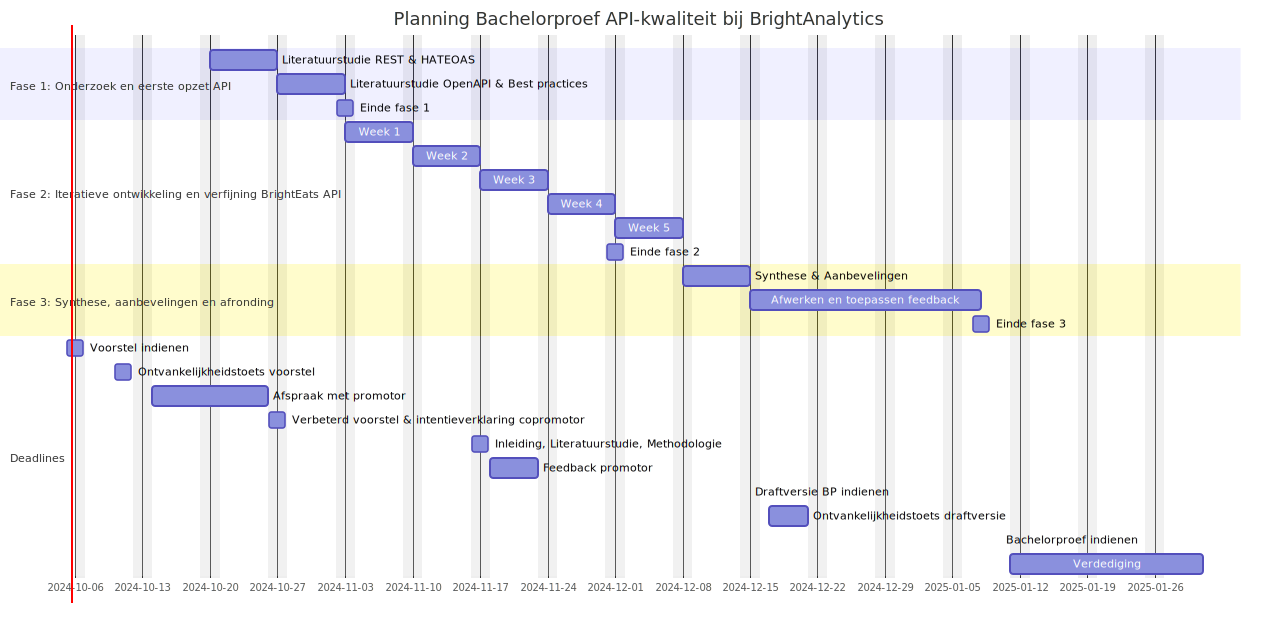
\includegraphics[width=\textwidth, keepaspectratio]{gantt-chart/gantt-chart.png}
  \caption{Gantt chart van de planning van de bachelorproef}
  \label{fig:gantt-chart}
\end{figure}
